\documentclass[conference]{IEEEtran}
\usepackage{enumitem}
\usepackage{amsmath}
\usepackage{cite}
\usepackage{graphicx}
\graphicspath{ {./}{./images/} }

\title{PCA-Based Image Compression}

\author{
\IEEEauthorblockN{Owen Sowatzke}
\IEEEauthorblockA{\textit{Electrical Engineering Department} \\
\textit{University of Arizona}\\
Tucson, USA \\
osowatzke@arizona.edu}
\and
\IEEEauthorblockN{Scott Thoesen}
\IEEEauthorblockA{\textit{Electrical Engineering Department} \\
\textit{University of Arizona}\\
Tucson, USA \\
thoesens@arizona.edu}}

\begin{document}
    \maketitle
		
    \section{Introduction}
    This project aims to explore principle component analysis (PCA), its relationship to singular value decomposition (SVD), and its application to the field of image compression \cite{jaradet_svd_image_compression}. The topic of digital image compression has become more important than ever with the advent of smartphones and social media, with millions of images created, stored, transferred, and copied daily. Reducing the digital footprint of this data is therefore necessary to both satisfying end-user demands and decreasing the demand on limited computing and storage resources. Although image compression is interesting and generally important, it is not of particular importance to the authors. What is important to the authors is the more generalized use of PCA as a tool for data analysis and dimensionality reduction. Image compression was selected for this project to visually demonstrate the connection that is made by PCA between real-world data and linear algebra.

    \section{Background}
    PCA was not explicitly covered in ECE 501b but its underlying machinery, the SVD was. An entire lecture was dedicated to covering the SVD, which is an accumulation of many core concepts learned throughout the semester. The SVD employs many linear algebra concepts including inner product spaces, the null space, injectivity and surjectivity, dimensionality, linear independence, bases, orthonormality, linear maps, eigenvalues and eigenvectors, adjoints of linear maps, square roots of linear maps, matrix representations of linear maps, matrix decomposition, diagonal matrices, square matrices, unitary and orthonormal matrices. These concepts will appear throughout this paper and are assumed to be known by means of ECE 501b lectures. External references will therefore not be provided since the implication is that ECE 501b lectures are the references.

    \subsection{Motivation}
    Digital images are signals, or vectors, which means they can be represented in various ways on different bases. Any basis is a collection of linearly independent vectors or functions that completely describe the vector space in which they are defined. Vectors, or signals, can therefore be represented on a basis as a linear combination of the constituent basis vectors. This representation is shown in Equation \ref{eq:basisdef}

    \begin{equation}
        v = \sum_{i=1}^{n} a_i \mathbf{\phi}_{i}
    \label{eq:basisdef}
    \end{equation}

    where $v$ is a vector, $a_i$ is a scalar, $\mathbf{\phi}_{i}$ is a basis vector or basis function, and $n$ is the length of the basis.

    Vectors in one basis can be converted to another by means of a linear transformation. Inverse operations also exist. Additionally, where a signal tends to be dense and feature rich in one basis, it is often sparse in another. When a basis is identified such that a sparse representation is possible, content that contains little to no information about the signal can be readily discarded. This leads to the intuition that signals are \textit{compressible}.

    Many compression techniques exist and fall into one of two categories: lossy and lossless. Lossless compression is concerned with the reduction of data size while maintaining the capacity to  completely recover the signal without degradation. Lossy compression concedes a level of irreversible degradation upon decompression. PCA-based compression is a lossy technique. Examples of other lossy compression schemes are JPEG, which employs the discrete cosine transform (DCT), and JPEG2000, which uses a wavelet transform (ref)(ref).
    
    Under special considerations, information lost during lossy compression does not imply a reduction of image quality. For example, the premise behind JPEG compression is the fact that the human visual 
    system cannot perceive high spatial frequencies beyond a certain limit. When the DCT of an image is computed, coefficients corresponding to frequency components beyond a certain threshold are discarded. The remaining lower-frequency components are retained and the image has been compressed. The decompressed image, obtained by an inverse DCT, is then indistinguishable from the original to a human observer.

    The DCT and other transforms involve bases that are independent of the data being transformed. This often leads to inefficient representations of a signal, and thus poor compressibility. One signal may appear to be sparse or compact in the new basis but a different signal remains dense and broadly distributed under the same transformation. JPEG exhibits this behavior when compressing natural versus synthetic images (ref).
    
    SVD-, or PCA-, representation uses a basis that is learned from the data itself. The basis vectors are therefore directly related to the structure of the signal and consequently form a more efficient representation. As will be shown in the Results section of this paper, the representation is also more compact.
    
    \subsection{Singular Value Decomposition}
    The Singular Value Decomposition Theorem states that for any matrix $\mathbf{A} \in \mathbf{F}^{n \times n}$, a unique representation of the form shown in equation (ref eq) exists [ref].

     \begin{equation}
     \mathbf{A} = \mathbf{U\Sigma }{\mathbf{V}^\mathbf{T}}
     \end{equation}

    where $\mathbf{A} \in \mathbf{F}^{m \times m}$ and $\mathbf{V} \in \mathbf{F}^{n \times n}$ are square unitary
    matrices whose columns represent the left singular vectors and right singular vectors, respectively, and $\mathbf{\Sigma} \in \mathbf{F}^{m \times n}$ is a matrix of zeros except for the elements of the main diagonal which are called singular values. The singular values of $\mathbf{A}$ are always non-negative and real. When $\mathbf{A}$ is a real matrix, $\mathbf{U}$ and $\mathbf{V}$ are real and thus orthonormal.

    A literal interpretation of the SVD is the action taken by a linear map split into three discrete operations. The first operation performs a rotation of a vector onto an orthonormal basis in the domain of the map. The second operation simultaneously scales the vector and potentially changes dimensionality. The final operation is a rotation onto an orthonormal basis in the co-domain of the map.

    The SVD is a generalized analog of the eigendecomposition of a matrix, which is a result of the Spectral Theorem for certain linear operators, or square matrices (ref eigendecomp)(ref spectral). The eigenvectors of a full-rank normal operator, found through eigendecomposition, form an orthonormal basis on the inner product space of the operator called an eigenbasis. Thus, any vector in the inner product space can be represented completely and uniquely as an appropriate scaling of the eigenbasis vectors. The vectors of an eigenbasis are also called the modes of the operator. The magnitude of the eigenvalue associated with each mode determines the relative importance, or significance, of the mode. Modes with higher importance, or larger eigenvalues, contain more pertinent information about a vector than modes with smaller eigenvalues. In similar fashion, the right singular vectors of any operator represent the modes of the operator in the domain and the left singular vectors represent the modes in the co-domain. The magnitudes of the singular values determine the relative joint-importance, or joint-significance, of the associated singular vectors.
    
    \subsection{Principle Component Analysis} \label{pca_section}
    
    Using linear combinations of the existing basis, Principle Component Analysis (PCA) seeks to create a new basis which better represents the data \cite{shlens_2014_tutorial}. Let $\mathbf{X} \in \mathbf{F}^{m \times n}$ be a matrix of samples given with respect to the original basis, and let $\mathbf{Y} \in \mathbf{F}^{m \times n}$ be a matrix of samples given with respect to the updated basis. The operator $\mathbf{P} \in \mathbf{F}^{m \times m}$ re-expresses the samples in $\mathbf{X}$ in terms of an updated basis, resulting in $\mathbf{Y}$.
    
    \begin{equation}
    		\mathbf{Y} = \mathbf{P^{H}X}
    \end{equation}
    
    Let $\mathbf{p_i}$ for $i = 1,...,m$ be the columns of $\mathbf{P}$. The vectors $\{\mathbf{p_1},...,\mathbf{p_m}\}$ are the principal components of $\mathbf{X}$. The principle components are orthonormal vectors which maximize sample variance \cite{shlens_2014_tutorial}. Let each column of $\mathbf{X}$ be denoted as $\mathbf{x_j}$ and each column of $\mathbf{Y}$ be denoted as $\mathbf{y_j}$ for $i = 1,...,n$. Each vector $\mathbf{x_j}$ can be written as a linear combination of the basis vectors $\mathbf{p_1},...,\mathbf{p_m}$.
    %
    \begin{equation}
        \mathbf{x_j} = \langle \mathbf{x_j}, \mathbf{p_1}\rangle \mathbf{p_1} + \cdots + \langle \mathbf{x_j}, \mathbf{p_m}\rangle \mathbf{p_m}
    \end{equation}
    %
    Each coordinate in $\mathbf{y_j}$ is the scaling applied to the corresponding basis vector.
    	
    \begin{equation}
        \mathbf{y_j} = \begin{bmatrix}
                        \langle \mathbf{x_j}, \mathbf{p_1} \rangle\\
                        \vdots \\
                        \langle \mathbf{x_j}, \mathbf{p_m}\rangle
                        \end{bmatrix}
    \end{equation}
    	
    	
    %TALK ABOUT PCA HERE
    %How does the selected material for your project relate to SVD?
    %Theory of compression using PCA


    \section{Results}

    The compression technique described in Section \ref{pca_section} is implemented in Matlab. The Matlab built-in image 'wagon.jpg' is used throughout this section as an example for both qualitative and quantitative analysis of the compression scheme. Qualitative analysis is performed through visual inspection of image quality after compression. Quantitative analysis is performed by examining the peak signal-to-noise ratio (PSNR) of the compressed image, compared to the original, uncompressed image.

    \subsection{Data}
    Talk about image properties here, including size and format.

    \subsection{Design}
    Describe what the Matlab code is doing here. Talk about the color space conversion too.

    \subsection{Analysis}
    As mentioned in Section \ref{pca_section} every matrix can be decomposed into a linear combination of its modes. The relative importance, or significance, of a mode is determined by the magnitude of its associated singular value. A digital image is represented by a matrix and is therefore decomposed in the same way. In the context of image decomposition, the magnitude of each singular value determines the relative quantity of image information present in the respective modes.

    \begin{figure}[t]
    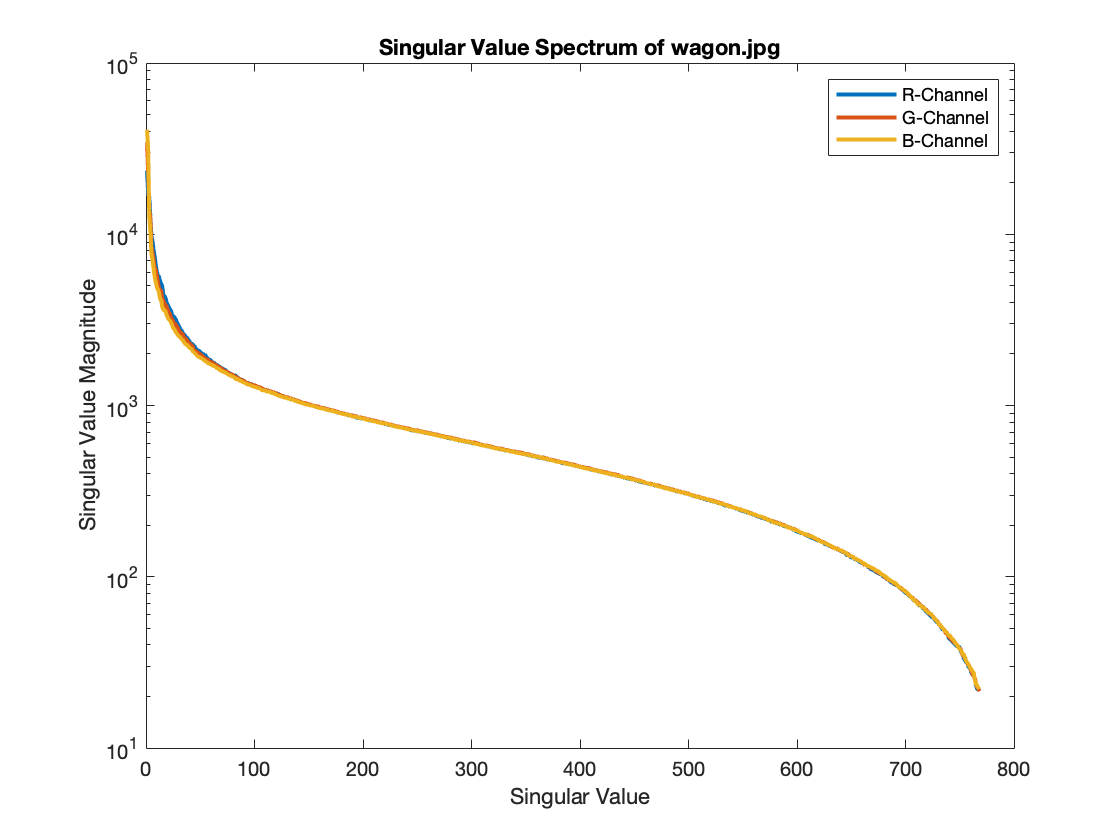
\includegraphics[width=0.5\textwidth]{svals_wagon_rgb}
    \caption{Plot showing the singular values of wagon.jpg. The SVD is computed separately for the red (R), green (G), and blue (B) channels}
    \label{fig:svalplot}
    \end{figure}
    
    Shown in Figure \ref{fig:svalplot} is a plot of the singular values of the image wagon.jpg. Of particular note is the low number of large singular values, approximately 100, compared to the total of 768. This concentration of large singular values suggests the majority of the modes contain little information about the image. Thus, removing modes associated with small singular values agrees with the intuition that images can be reduced in size while preserving the majority of the information content. Since the image is completely defined by the combination of all modes, the sum total of the singular values can be seen as an analog for the total information, or energy, contained in the image. Figure \ref{fig:svalenergyplot} shows the accumulation of energy as the number of modes representing the image increases from most to least significant. For example, to represent 80\% of the content of the image, the first 300 modes are needed.

    \begin{figure}[t]
    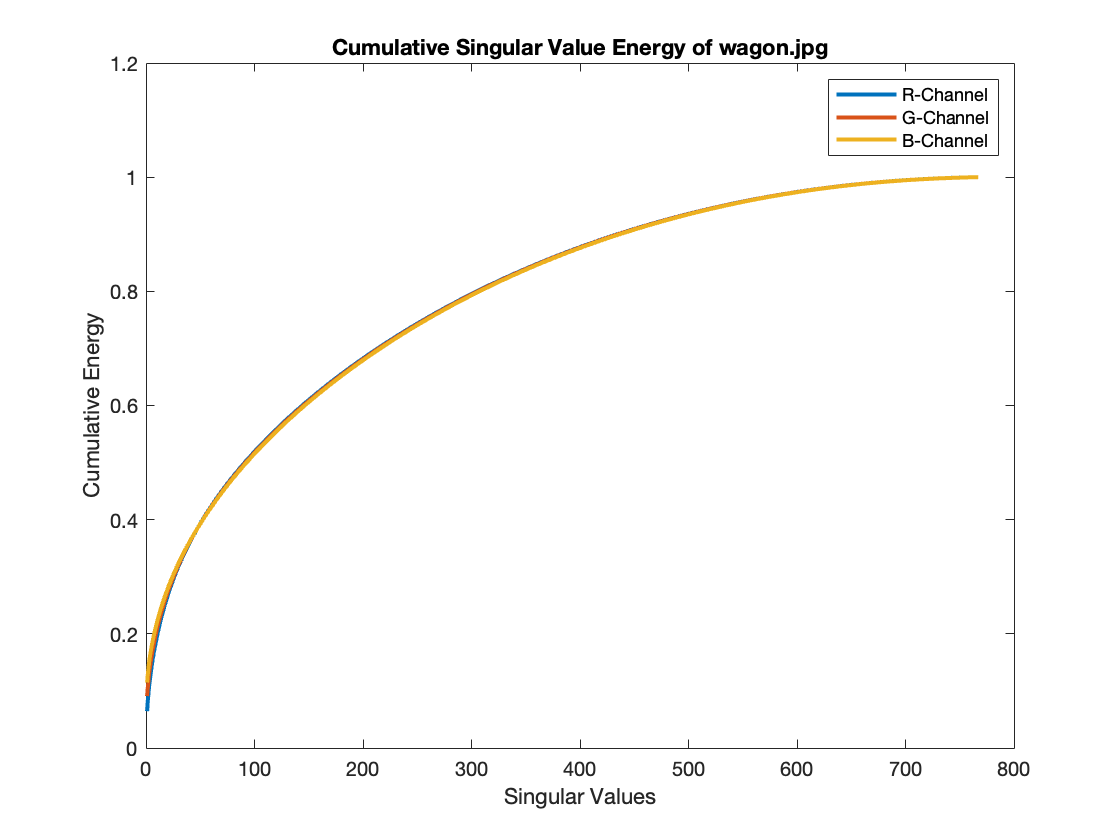
\includegraphics[width=0.5\textwidth]{sv_energy_wagon_rgb}
    \caption{Plot showing the cumulative energy of the singular values of wagon.jpg. Cumulative energy is computed separately for the red (R), green (G), and blue (B) channels}
    \label{fig:svalenergyplot}
    \end{figure}
    
    \begin{figure}[t]
    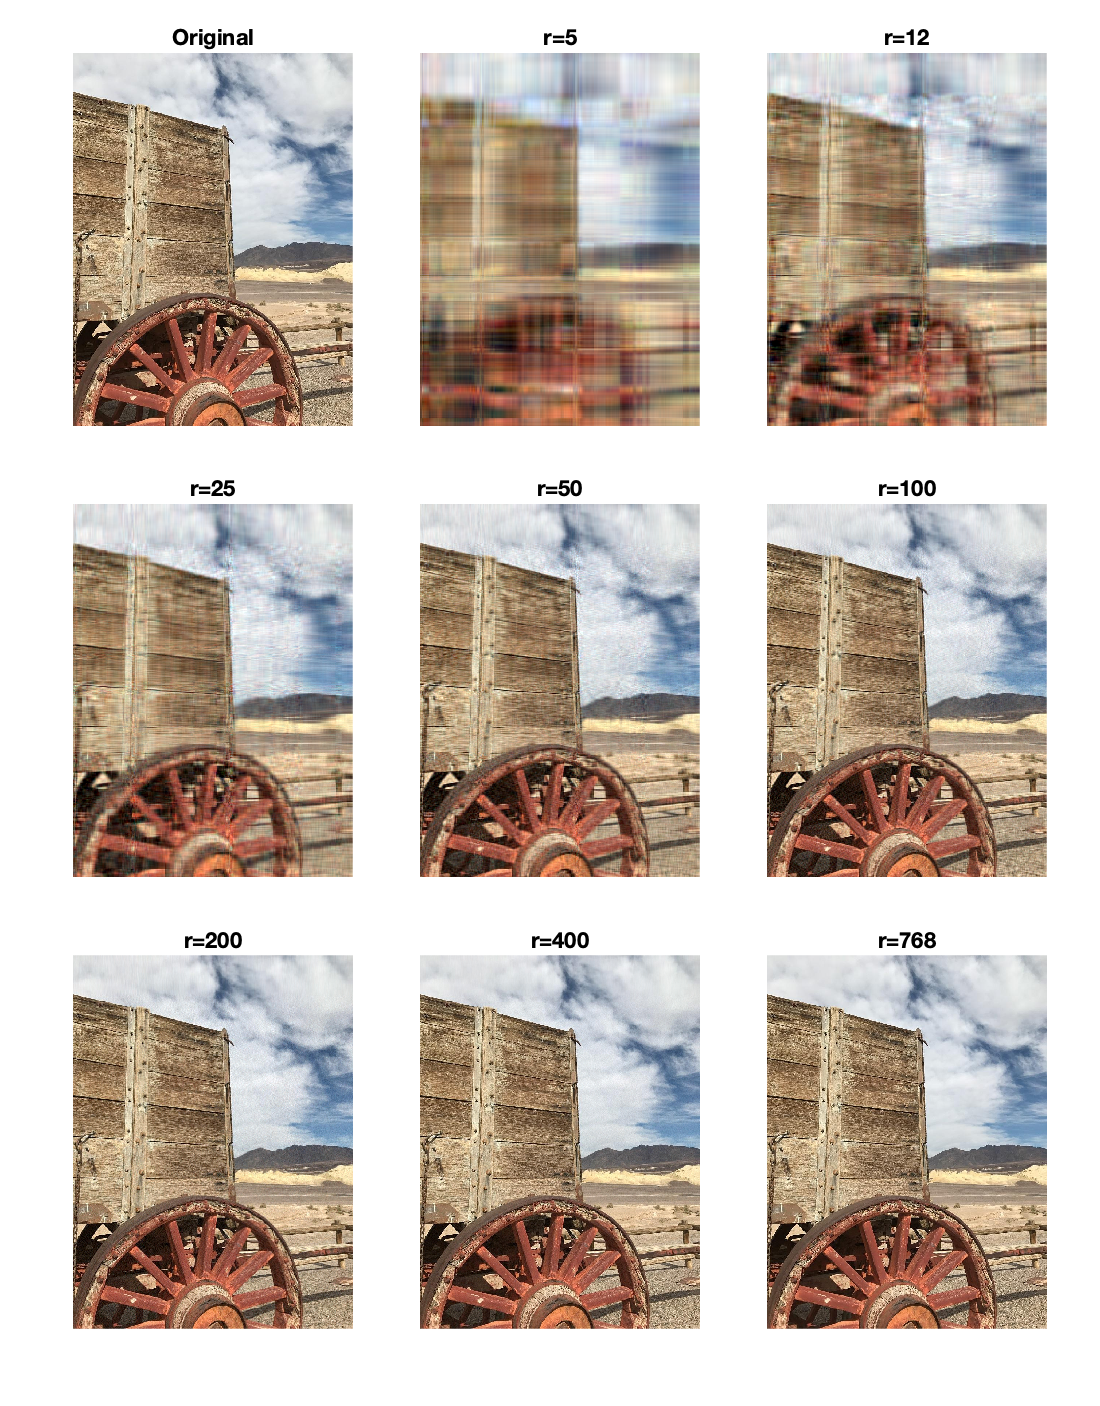
\includegraphics[width=0.5\textwidth]{show_different_r_wagon}
    \caption{Wagon wheel image using various numbers of representative modes}
    \label{fig:showwagondiffr}
    \end{figure}

    The effect of additional modes can be seen in Figure \ref{fig:showwagondiffr}. There are clear signs of distortion when the number of representative modes is low, in the range of 10-20, but distortion appears to fade as the number of modes reaches 200-400. According to the cumulative energy plot in Figure \ref{fig:svalenergyplot}, this level of compression retains 68\% to 88\% of the information content of the image. A more quantitative measure of compressed image quality is peak signal-to-noise ratio (PSNR), defined in Equation \ref{eq:psnr}

    \begin{equation}
    		PSNR = 10log_{10}(\frac{peakval^2}{MSE})
    \label{eq:psnr}
    \end{equation}

    where $peakval$ is the maximum representable value of the image's datatype and $MSE$ is the mean squared error between the compressed image and original, uncompressed image.

    Figure \ref{fig:psnrvsr_wagon} shows a plot of PSNR versus number of modes representing the wagon image. PSNR rises rapidly for the first few modes, then steadily for the total number of modes ranging from ~100 to ~550, then rapidly again as the decompressed image approaches the true image in value. Theoretical PSNR for a perfect reconstruction is infinity but is unlikely to be achieved due to quantization error. According to \cite{psnr_quality} typical PSNR values for high quality lossy reconstruction of an 8-bit image are 30-50dB. This agrees with our results which show a PSNR range of 27-34dB for 200-400 modes.

    \begin{figure}[t]
    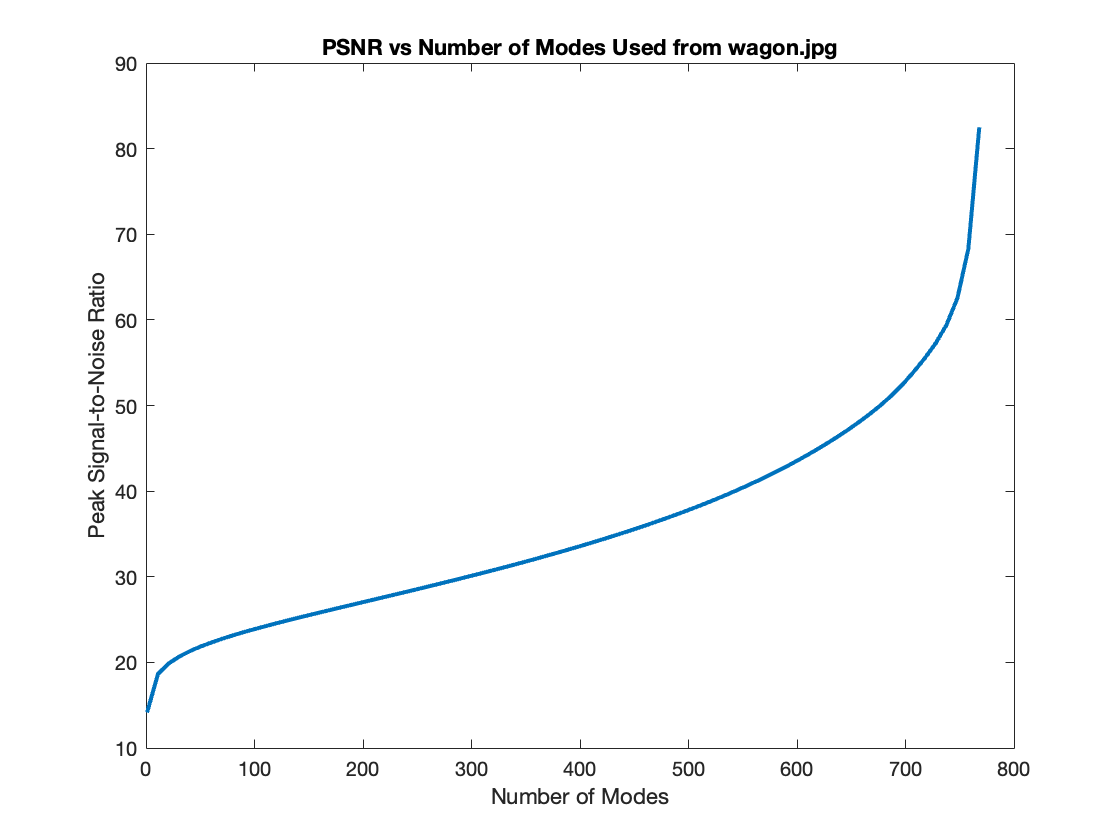
\includegraphics[width=0.5\textwidth]{snrvsr_wagon_rgb}
    \caption{Peak signal-to-noise ratio versus total number of modes}
    \label{fig:psnrvsr_wagon}
    \end{figure}
    
    Retaining the first 200-400 modes would suggest, at least from a subjective perspective, that the image can be reduced in size by a factor of 1.92 to 3.84. According to the plot in Figure (ref; show compression ratio vs r), the computed compression ratio for 100-200 modes is between X and Y.

    % Add Compression ratio vs R plot

    % Add comments about the differences between the Y and Cb/Cr curves?

    %Using the 25,000,000,000 Eigenvector paper as a guide, develop some exercises, questions, analysis, or examples that were inspired or motivated by your project. For example, what assumptions were made in your project material? What if certain assumptions are neglected or do not exist? Can you provide analysis that supplements the analysis in the selected project material Or, can you provide analysis that extends the analysis in the project material You might also develop numerical examples that help to provide insight into the ideas discussed in the selected material or that demonstrate the application of the theory in your project. The example you create might consist of a MATLAB simulation or MATLAB analysis.


    \section{Conclusion}
    
    %Provide a summary and conclusion section in the report. How well did your example correlate or explain the concepts in the selected material? How would you modify your example to make it better? How did your selected project enhance your understanding of ECE 501b material?

    \nocite{jaradet_svd_image_compression}
    \nocite{shlens_2014_tutorial}
    \nocite{omar_image_compression}
    \nocite{xu_color_conversion}
    \newpage
    \bibliography{sources}{}
    \bibliographystyle{ieeetr}
\end{document}
